\section{Estimate branching fraction}
We assume that $D_{s}^{+} \rightarrow X(p\bar{p}) e^{+} \nu_{e}$ and $p
\bar{p}$ from $X(p\bar{p})$, where $X(p\bar{p})$ is a pseudo-scalar meson. The
width of decay is $q^{2}$ dependence: 

\begin{equation}
    \frac{d \Gamma (D_{s}^{+} \rightarrow X e^{+} \nu _{e} )}{d q^{2}}
    = \frac{G^{2}_{F} \cdot | V_{cs} |^{2} p_{X} ^{3} }{24 \pi ^{3}} f
    _{X} (q^{2})^{2} 
\end{equation}
where the form factor is assumed different function of $q^{2}$ in
different model. 

We compare the decay width between $D_{s}^{+} \rightarrow \eta e^{+}
\nu_{e}, X(p\bar{p}) e^{+} \nu_e{e}$ to get the branching fraction:
    
\begin{equation}
    Br(D_{s}^{+} \rightarrow X(p\bar{p}) e^{+} \nu_{e}) = Br(D_{s}^{+}
    \rightarrow \eta e^{+} \nu_{e}) \frac{\Gamma_{X}}{\Gamma_{\eta}}
\end{equation}

Assume\cite{Bauer:1988fx}: 
\begin{equation}
    f(q^{2}) = \frac{f_{0}}{1-\frac{q^{2}}{M_{pole}^{2}}}
\end{equation}
where $f_{0}$ is about 0.5, and $M_{pole} \sim m_{D_{s}^{+}}$.

The branching fraction is not sensitive to $M_{pole}$, but strongly
relies on the parameter $f_{0}$ as shown in Fig. \ref{Fig: float
parameter}. We assign 1 to $f_{0}$ reasonably, and obtain the branching
fraction: 
\begin{equation}
Br(D_{s}^{+} \rightarrow X(p\bar{p}) e^{+} \nu_{e}) \sim
10^{-5}  \notag
\end{equation}
\begin{figure}[htbp]
    \center{
        \mbox{
            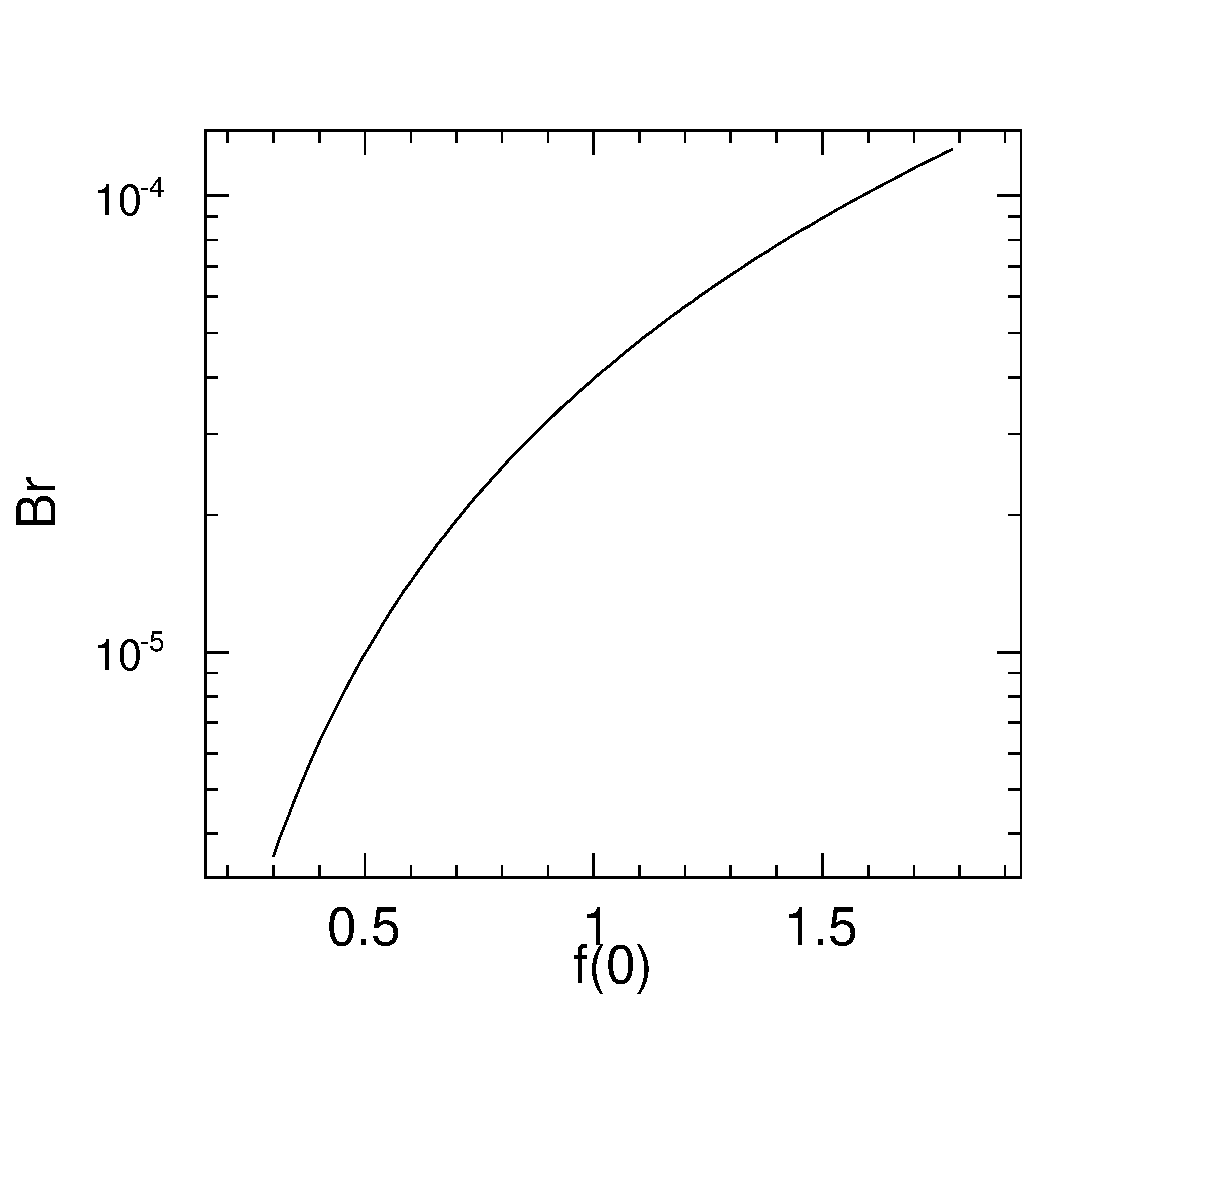
\includegraphics[width=5cm]{section/append/fig/f_0.eps}
            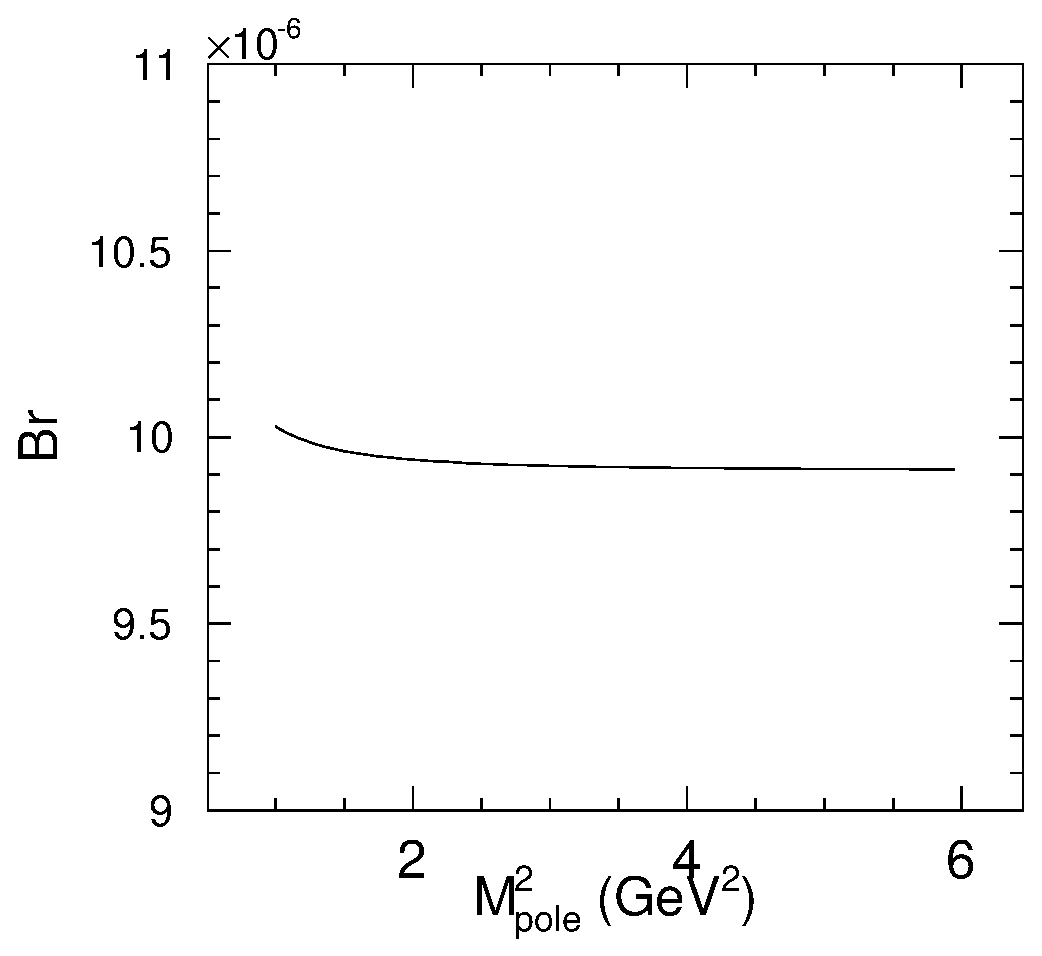
\includegraphics[width=5cm]{section/append/fig/m_pole.eps}
        }
    }
    \caption{Float the parameter $f(0)$ and $M_{pole}^{2}$ }
    \label{Fig: float parameter}
\end{figure}
    
